%%%%%%%%%%%%%%%%%%%%%%% file template.tex %%%%%%%%%%%%%%%%%%%%%%%%%
%
% This is a general template file for the LaTeX package SVJour3
% for Springer journals.          Springer Heidelberg 2010/09/16
%
% Copy it to a new file with a new name and use it as the basis
% for your article. Delete % signs as needed.
%
% This template includes a few options for different layouts and
% content for various journals. Please consult a previous issue of
% your journal as needed.
%
%%%%%%%%%%%%%%%%%%%%%%%%%%%%%%%%%%%%%%%%%%%%%%%%%%%%%%%%%%%%%%%%%%%
%
% First comes an example EPS file -- just ignore it and
% proceed on the \documentclass line
% your LaTeX will extract the file if required
\begin{filecontents*}{example.eps}
%!PS-Adobe-3.0 EPSF-3.0
%%BoundingBox: 19 19 221 221
%%CreationDate: Mon Sep 29 1997
%%Creator: programmed by hand (JK)
%%EndComments
gsave
newpath
  20 20 moveto
  20 220 lineto
  220 220 lineto
  220 20 lineto
closepath
2 setlinewidth
gsave
  .4 setgray fill
grestore
stroke
grestore
\end{filecontents*}
%
\RequirePackage{fix-cm}
%
%\documentclass{svjour3}                     % onecolumn (standard format)
%\documentclass[smallcondensed]{svjour3}     % onecolumn (ditto)
\documentclass[smallextended]{svjour3}       % onecolumn (second format)
%\documentclass[twocolumn]{svjour3}          % twocolumn
%
\smartqed  % flush right qed marks, e.g. at end of proof
%

\usepackage{graphicx}
\usepackage{amsmath}
\usepackage{algorithm}
\usepackage{algorithmic}
\usepackage{tikz}
\renewcommand{\algorithmicrequire}{\textbf{Initialize:}}

\usepackage{verbatim} %TODO delete before submission
\usepackage[numbers]{natbib}%TODO delete before submission

%TODO Zitierweise ändern, sieht schrecklich aus
%
% \usepackage{mathptmx}      % use Times fonts if available on your TeX system
%
% insert here the call for the packages your document requires
%\usepackage{latexsym}
% etc.
%
% please place your own definitions here and don't use \def but
% \newcommand{}{}
%
% Insert the name of "your journal" with
% \journalname{myjournal}
%
\begin{document}

\title{Application of Reinforcement Learning Methods
%\thanks{Grants or other notes
%about the article that should go on the front page should be
%placed here. General acknowledgments should be placed at the end of the article.}
}
\subtitle{Group 19 - Final Project Report}

%\titlerunning{Short form of title}        % if too long for running head

\author{Yannik Frisch \and Tabea Wilke \and Maximilian Gehrke %etc.
}

\maketitle

\section{Introduction}
\label{sec:intro}
We shortly present two state-of the art reinforcement learning algorithms, the \textit{Deep Deterministic Policy Gradient} and the \textit{Natural Actor Critic}. Both algorithms are evaluated on the simulated Quanser Robots platforms \textit{BallBalancerSim-v0}, \textit{CartPoleStabShort-v0} and \textit{Qube-v0}. We furthermore present the results of training both algorithms on the \textit{BallBalancerSim-v0} and evaluating it on the pyhiscal \textit{BallBalancerRR-v0} platform. Finally, we let a pretrained \textit{Natural Actor Critic} agent continue learning on the physical version of \textit{CartPoleStabShort-v0} and close with a discussion of the results.
\newpage
\section{Deep Deterministic Policy Gradient}
\label{sec:ddpg}
The \textit{Deep Deterministic Policy Gradient} approach \citep{lillicrap2015continuous} is an application of the \textit{Deep Q-Learning} algorithm \citep{mnih2013playing} to actor-critic methods \citep{konda2000actor} in combination with the \textit{Deterministic Policy Gradient} \citep{silver2014deterministic}. It is a model-free and off-policy algorithm, learning a deterministic policy. We separated the learning process completely from the algorithm's other components. The critic is updated using the temporal difference error, calculated from using the target networks, which are constrained to slow changes with rate $\tau$ to improve the stability of learning. The actor is trained by using the integrated update rule from \cite{lillicrap2015continuous} as it's loss function. Both networks are addressed and can be modified in a separate file, same as the replay buffer, which is used to sample independently and identically distributed mini-batches, randomly selected to temporarily decorrelate them. The action noise to ensure exploration was also kept completely independent from the training algorithm as intended by \citep{lillicrap2015continuous} and is just added to the output of the actor. We clip this output to ensure it suits the environment.

\subsection{Evaluation on BallBalancerSim-v0}
The Quanser Robots \textit{BallBalancerSim-v0} environment consist of a plate whose angles can be controlled by the input actions. The goal is to balance a ball on the plate, receiving a maximum reward of 1.0 per time-step for balancing it in the middle of the plate. The environment ends after a maximum of 1000 time-steps.\\
We started our evaluations with using two hidden layers with 100 and 300 hidden neurons for the actor and the critic networks and their targets. The learning rates are set to $\alpha_{actor}=1e-4$ and $\alpha_{critic}=1e-3$. 
In the left row of figure \ref{ddpg:ball} one can find our first acceptable results. Discounting is set to $\gamma=0.99$, we did soft target updates with $\tau=1e-4$, used a mini-batch size of 64 and a total replay buffer size of 1e6. We slightly increased the noise to $\sigma_{OU}=0.2$ and $\theta_{OU}=0.25$ as the environments action space has an higher amplitude compared to the \textit{Pendulum-v0} trained on in \citep{lillicrap2015continuous}.\\
The algorithm did learn to balance the ball, but was not very stable, which can also be read from the learning progress plot. To further increase the stability, we increased th mini-batch size used to sample from the replay buffer, and reduced the noise again. Using weight regularization did not seem to be helpful, so we set it to zero.\\
Figure \ref{ddpg:ball:gamma} shows the training process where discounting is set to $\gamma=0.2$ compared to $\gamma=0.99$. One can see discounting is crucial to solve this environment.\\
\begin{figure}[H]
	\centering
	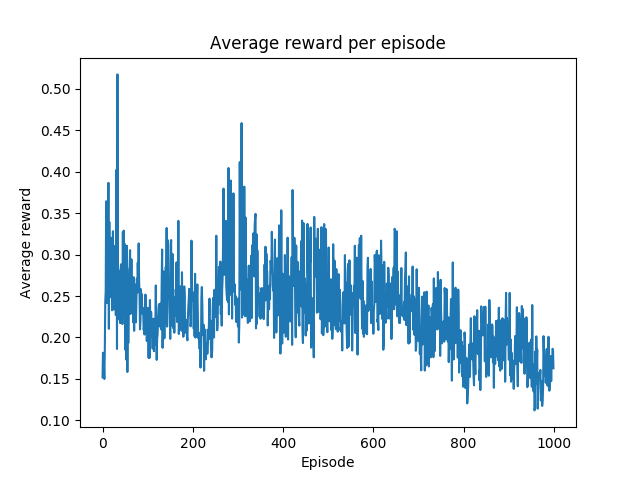
\includegraphics[width=0.4\textwidth]{plots/ddpg_ball_low_gamma.png}
	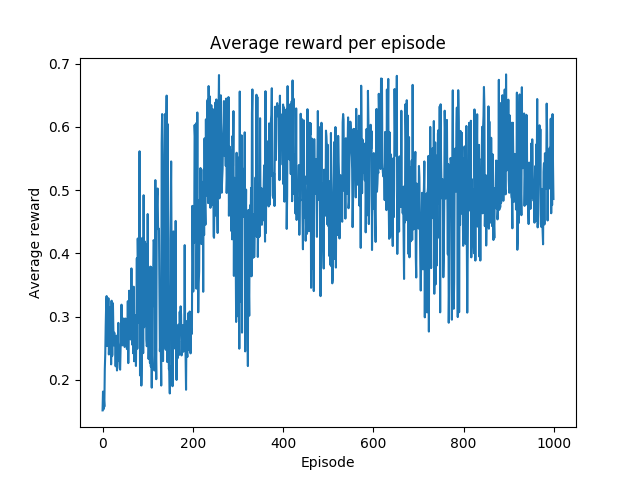
\includegraphics[width=0.4\textwidth]{plots/ddpg_ball_high_gamma.png}
	\caption{The left figure shows the cumulative reward per episode during the training process with $\gamma$ set to 0.2. The right one displays the process for $\gamma=0.99$. Using discounting close to 1 was very important.}
	\label{ddpg:ball:gamma}
\end{figure}
We tried to reduce the computational effort by only using a single hidden layer with 100 hidden neurons instead of two layers. The impact on the performance is shown in the middle row of figure \ref{ddpg:ball}. The learning suffered from instabilities, so we decided to weight the stability of using two hidden layers higher than the performance loss.\\
Our best results can be found in the right row of figure \ref{ddpg:ball} where we set the OU action noise equal to the one used in the original paper with $\sigma_{OU}=0.15$ and $\theta_{OU}=0.2$. We used slightly harder updates with $\tau=1e-3$, and achieved an average cumulative reward of about 650 for 25 episodes of evaluation. The learning process took about 3 hours for 1000 episodes. Further evaluations are needed to improve the training even more.
\begin{figure}[H]
	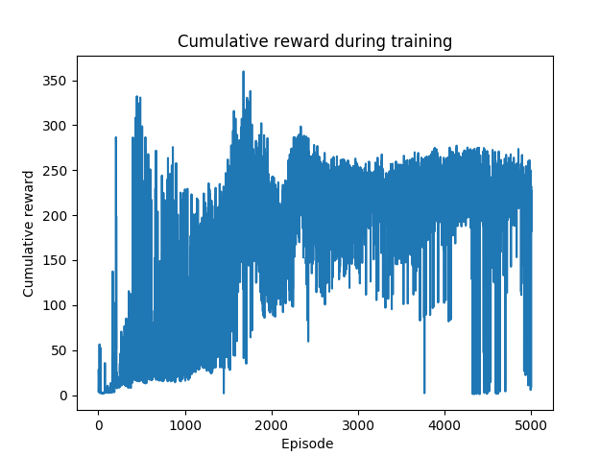
\includegraphics[width=0.325\textwidth]{plots/ddpg_ball_first_train.png}
	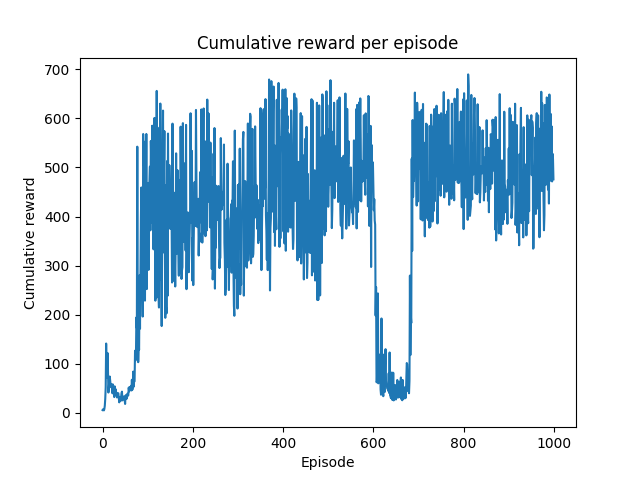
\includegraphics[width=0.325\textwidth]{plots/ddpg_ball_1layer_train.png}
	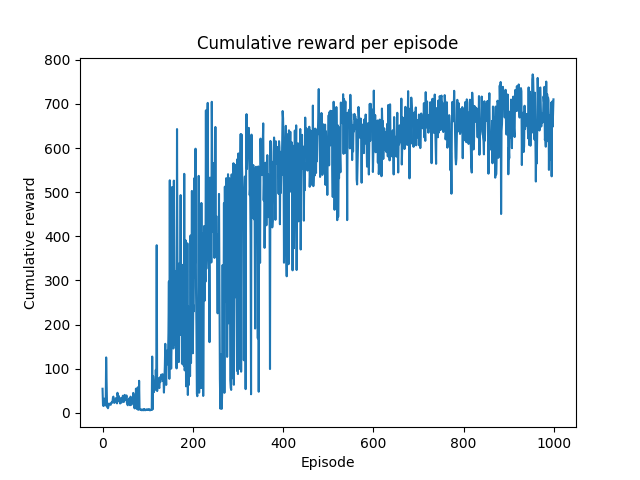
\includegraphics[width=0.325\textwidth]{plots/ddpg_ball_best_train.png}
	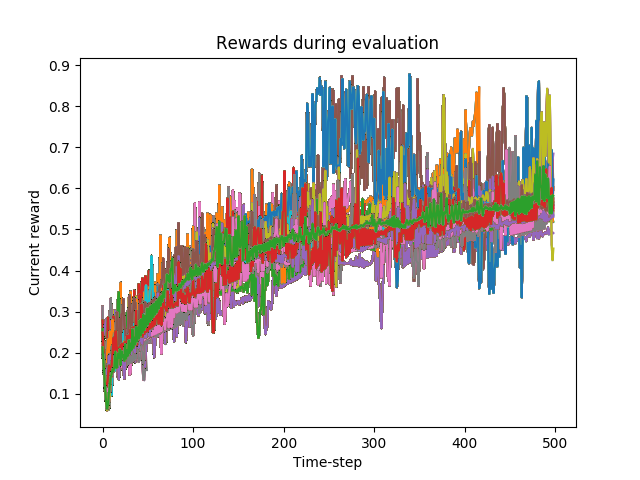
\includegraphics[width=0.325\textwidth]{plots/ddpg_ball_first_eval.png}
	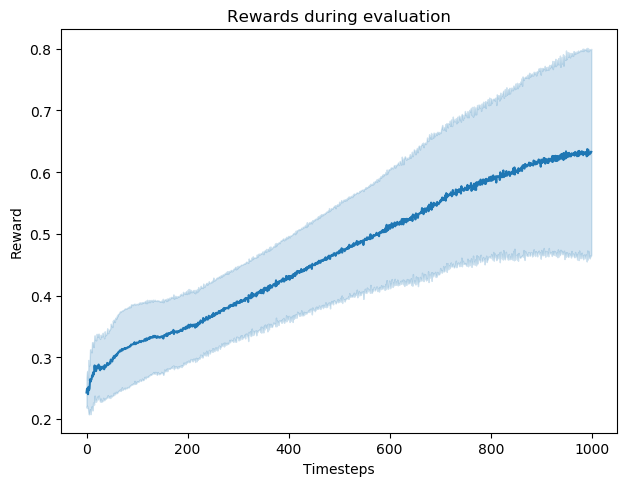
\includegraphics[width=0.295\textwidth]{plots/DDPGballbalancer24-2-16.png}
	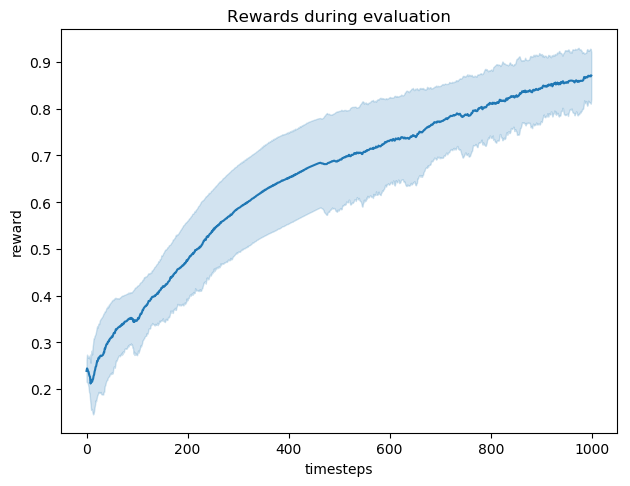
\includegraphics[width=0.295\textwidth]{plots/DDPGballbalancer26-2-20.png}

	\caption{The figure displays the training process in the first row and the evaluation results in the second row. Early learning successes can be found in the left column, while the middle column shows the influence of using only a single hidden layer. The right column gives the plots of our best training result.[EDIT: ALIGN PLOTS + LEFT PLOT IS WRONG (WRONG ENV...)]}
	\label{ddpg:ball}
\end{figure}
\subsection{Evaluation of the Pretrained Model on the Real Ball Balancer System}
Evaluating our best model trained in simulation on the real ball balancer was not successful. The chosen actions were too big and the plate instantly tilted. Also, it was not possible for us to reset the environment between the evaluation episodes. The result of single episodes of evaluation can be found in figure [x].
\subsection{Evaluation on CartPoleStabShort-v0}
The Quanser Robots \textit{CartPoleStabShort-v0} environment consists of a movable car with a singular pendulum attached. The car can be controlled by input actions. The goal is to balance the pendulum, starting from a vertical position and the reward is depending on the angle, with a maximum of 2.0 per time-step for balancing the pendulum straight upright.\\
We achieved some progress using [x]. The results are displayed in [x].
\subsection{Evaluation on Qube-v0}
The Quanser Robots \textit{Qube-v0} environment implements the Furuta Pendulum, which consists of a motor controlling one horizontal arm. One end of the joint is attached to the motor, the other end is attached to another vertical arm, which can only be controlled indirectly by controlling the first arm. More details about the Furuta Pendulum can be found in our paper about it.\\
The goal is to balance the second arm in upright position, receiving a maximum reward of 0.02 per time-step. The environment stops after 300 time-steps.
We did not get any useful results re-using the parameters we found for \textit{BallBalancer-v0}. Using an Ornstein Uhlenbeck similar to the one used in citep{lillicrap2015continuous}, did not seem to help to deal with the local optima of the environment. Setting the randomness $\sigma_{OU}$ too small resulted in too less exploration. Choosing a higher $\sigma_{OU}$ resulted in better exploration but much less stability. Examples are displayed in figure \ref{ddpg:qube}.\\
No stable training process could be achieved. To address this issue we started using a consistent gaussian noise. Unfortunately this did also not help the training process, and seemed to be even more unstable. Figure \ref{ddpg:qube} shows a result of using gaussian noise in the right plot. The algorithm seemed to learn well for a period of time, but tended to overwrite these progress. Lowering the target update rate $\tau$ did not help, nether did lowering the actor and critic learning rates.
\begin{figure}[H]
	\begin{center}
	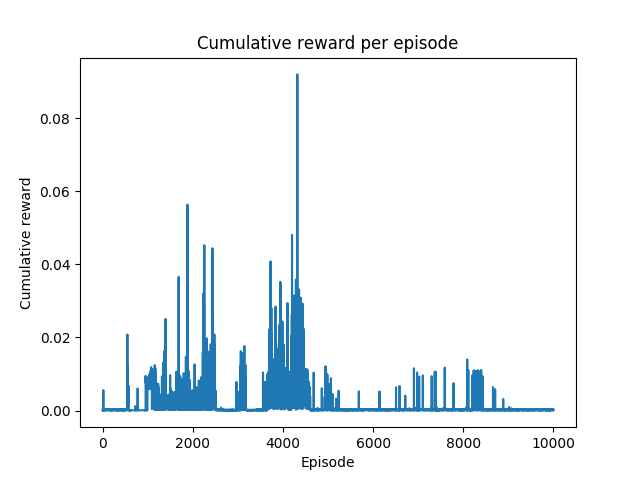
\includegraphics[width=0.325\textwidth]{plots/ddpg_qube_ou_bad_train.png}
	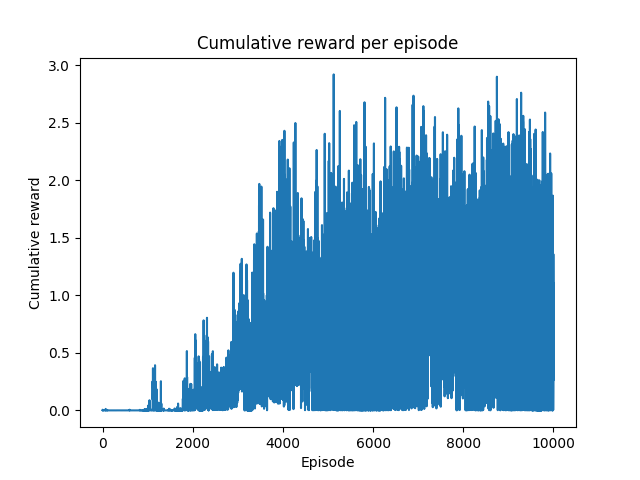
\includegraphics[width=0.325\textwidth]{plots/ddpg_qube_ou_better_train.png}
	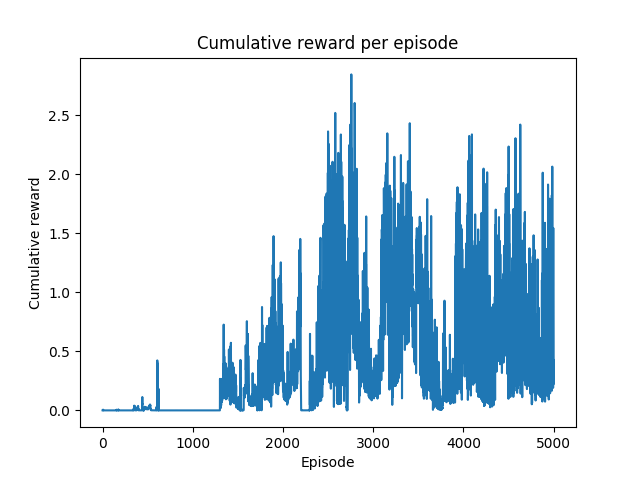
\includegraphics[width=0.325\textwidth]{plots/ddpg_qube_gauss.png}
	\caption{Assuming the parameters from our best result on \textit{BallBalancerSim-v0}, we achieved the performance shown in the left plot on \textit{Qube-v0}. The middle plot shows the changes when using more OU noise, i.e. $\sigma=3.2$. The right plot displays the result of training with a gaussian noise with mean zero and 
	standard deviation $\sigma=0.7$. The mini-batch size was also increased to 
	256.}
	\label{ddpg:qube}
\end{center}
\end{figure}
Our experiments induced several things: Using a higher batch size seemed to increase the stability to a certain level, but also highly increased the computational effort. 256 seemed to be a good batch-size. The decisions harder or softer updates, controlled by $\tau$, and the amount of action noise for exploration seemed to be very important but also very hard to tune. E.g. choosing $\tau=1e-2$ resulted in an agent tending to overwrite what he already learned, while setting $\tau=1e-4$ prevented him from learning anything. So we chose $\tau=1e-3$, but this alone was not sufficient for effective learning. Reducing the action noise added to the actor output did also not help. Further evaluations are needed to find the right set of hyper-parameters for this environment. 
\section{Natural Actor Critic}
\label{sec:nac}
\subsection{Evaluation on CartPoleSwingShort-v0}
\subsection{Evaluation on the BallBalancerSim-v0}
\subsection{Evaluation of the Pretrained Model on the Real Ball Balancer System}
\subsubsection{Learning from the Physical Cart Pole System with pretrained parameters}

\section{Discussion}
We implemented the DDPG and NAC algorithms and evaluated them on the Quanser Robots environments \textit{BallBalancerSim-v0}, \textit{CartPoleStabShort-v0} and the \textit{Qube-v0}. Both algorithms were able to learn a well performing policy for the first two environments, where the NAC needed less computational time and was more sample efficient. Nonetheless, both algorithms did have troubles to learn a close to optimal policy for the \textit{Qube-v0} environment. They suffered from a very difficult exploration / exploitation trade-off, often with stable learning in the beginning which is overwritten later, or not having enough exploration drive to escape local optima. Further evaluation is needed to optimize the algorithms especially for this environment. Due to technical difficulties it was not really possible to evaluate our pretrained models on the real Quanser Robots systems. Further investigation is needed.
\label{sec:conclusion}






\begin{comment}

We propose several possible extensions and show their performance on a task.\\
Text with citations \cite{RefB} and \cite{RefJ}.
\subsection{Subsection title}
\label{sec:2}
as required. Don't forget to give each section
and subsection a unique label (see Sect.~\ref{sec:1}).
\paragraph{Paragraph headings} Use paragraph headings as needed.
\begin{equation}
a^2+b^2=c^2
\end{equation}

% For one-column wide figures use
\begin{figure}
% Use the relevant command to insert your figure file.
% For example, with the graphicx package use
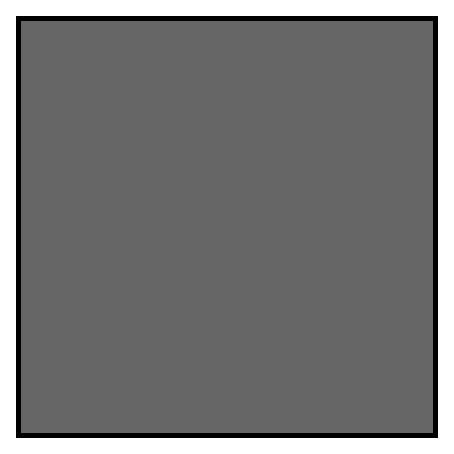
\includegraphics{example.eps}
% figure caption is below the figure
\caption{Please write your figure caption here}
\label{fig:1}       % Give a unique label
\end{figure}
%
% For two-column wide figures use
\begin{figure*}
% Use the relevant command to insert your figure file.
% For example, with the graphicx package use
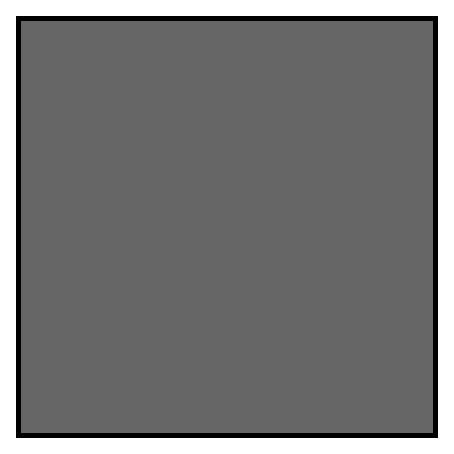
\includegraphics[width=0.75\textwidth]{example.eps}
% figure caption is below the figure
\caption{Please write your figure caption here}
\label{fig:2}       % Give a unique label
\end{figure*}


%
% For tables use
\begin{table}
% table caption is above the table
\caption{Please write your table caption here}
\label{tab:1}       % Give a unique label
% For LaTeX tables use
\begin{tabular}{lll}
\hline\noalign{\smallskip}
first & second & third  \\
\noalign{\smallskip}\hline\noalign{\smallskip}
number & number & number \\
number & number & number \\
\noalign{\smallskip}\hline
\end{tabular}
\end{table}


\end{comment}
%\begin{acknowledgements}
%If you'd like to thank anyone, place your comments here
%and remove the percent signs.
%\end{acknowledgements}

% BibTeX users please use one of
\bibliographystyle{spbasic}      % basic style, author-year citations
%\bibliographystyle{spmpsci}      % mathematics and physical sciences
%\bibliographystyle{spphys}       % APS-like style for physics
\bibliography{project_report.bib}   % name your BibTeX data base

% Non-BibTeX users please use
\begin{comment}


\begin{thebibliography}{}
%
% and use \bibitem to create references. Consult the Instructions
% for authors for reference list style.
%
\bibitem{RefJ}
% Format for Journal Reference
Author, Article title, Journal, Volume, page numbers (year)
% Format for books
\bibitem{RefB}
Author, Book title, page numbers. Publisher, place (year)
% etc

\end{thebibliography}
\end{comment}
\end{document}
% end of file template.tex
